% !TeX root = RJwrapper.tex
\title{Reproducible Summary Tables with the gtsummary Package}
\author{by Daniel D. Sjoberg, Karissa Whiting, Michael Curry}

\maketitle

\abstract{
An abstract of less than 150 words.
}

\section{Introduction}

\section{Data Summaries}

To show use of gtsummary functions, we will use a simulated clinical trial data set containing baseline characteristics of 200 patients who received Drug A or Drug B as well as the outcome of tumor response to the treatment.
Each variable in the data frame has been assigned an attribute label (i.e. \texttt{attr(trial\$trt, "label") == "Chemotherapy Treatment"}) with the labelled package\citep{labelled}. 
These labels are displayed in the {gtsummary} tables by default. Using {gtsummary} on a data frame without labels will print variable names in place of variable labels with the option to update the text displayed.

% adding table describing trial dataset
\captionsetup[table]{labelformat=empty,skip=1pt}
\begin{longtable}{llll}
\toprule
colname & label & class & values \\ 
\midrule
\texttt{trt} & Chemotherapy Treatment & character & \texttt{Drug A}, \texttt{Drug B} \\ 
\texttt{age} & Age & numeric & \texttt{6}, \texttt{9}, \texttt{10}, \texttt{17}, ... \\ 
\texttt{marker} & Marker Level (ng/mL) & numeric & \texttt{0.003}, \texttt{0.005}, \texttt{0.013}, \texttt{0.015}, ... \\ 
\texttt{stage} & T Stage & factor & \texttt{T1}, \texttt{T2}, \texttt{T3}, \texttt{T4} \\ 
\texttt{grade} & Grade & factor & \texttt{I}, \texttt{II}, \texttt{III} \\ 
\texttt{response} & Tumor Response & integer & \texttt{0}, \texttt{1} \\ 
\texttt{death} & Patient Died & integer & \texttt{0}, \texttt{1} \\ 
\texttt{ttdeath} & Months to Death/Censor & numeric & \texttt{3.53}, \texttt{5.33}, \texttt{6.32}, \texttt{7.27}, ... \\ 
\bottomrule\caption{\label{tab:caption}Table 1. Example data frame, \texttt{trial}}\\

\end{longtable}



\subsection{\texorpdfstring{\texttt{tbl\_summary()}}{tbl\_summary()}}

The default output from \texttt{tbl\_summary()} is meant to be publication ready.
The \texttt{tbl\_summary()} function can take, at minimum, a data frame as the only input, and returns descriptive statistics for each column in the data frame.
This is often the first table of clinical manuscripts and describes characteristics of the cohort under study.
A simple example is shown below.
Notably, by specifying the \texttt{by=} argument, you can stratify the summary table. 
In the example below, we have split the table by the treatment a patient received. 

% code for basic tbl_summary()
\begin{example}
trial %>%
  select(age, grade, response, trt) %>%
  tbl_summary(by = trt)
\end{example}
\begin{figure}[h!]
  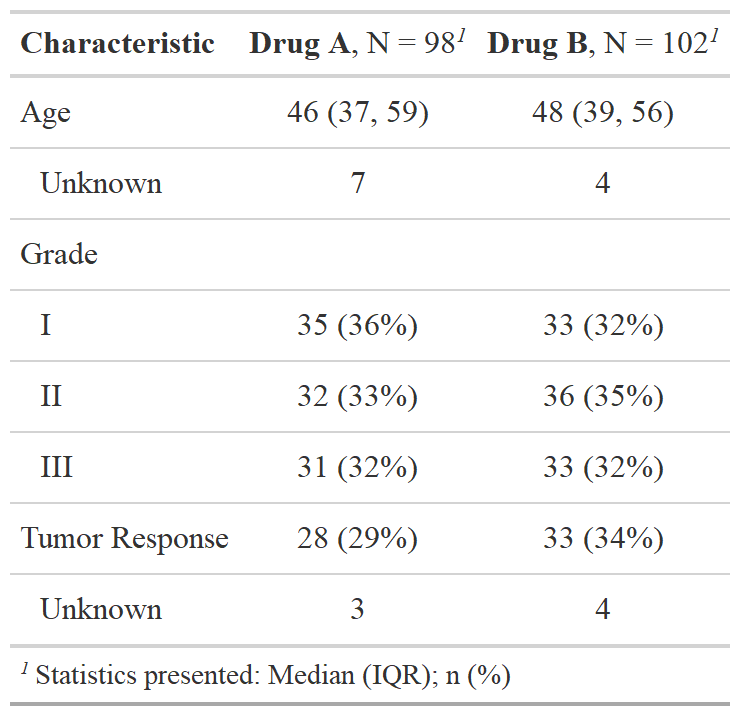
\includegraphics[height=5cm]{summary_basic.png}
  \centering
\end{figure}

The function is highly customizable, and it is initiated with sensible default settings.
Specifically, \texttt{tbl\_summary} detects variable types of input data and calculates descriptive statistics accordingly.
For example, variables coded as \texttt{0/1}, \texttt{TRUE/FALSE}, and \texttt{Yes/No} are presented dichotomously.
Additionally, \texttt{NA} values are recognized as missing and listed as unknown, and if a data set is labelled, the label attributes are automatically utilized. 

Default settings may be customized using the \texttt{tbl\_summary()} function arguments.

% code for tbl_summary() with arguments
\captionsetup[table]{labelformat=empty,skip=1pt}
\begin{longtable}{ll}
\toprule
Argument & Description \\ 
\midrule
\texttt{label=} & specify the variable labels printed in table \\ 
\texttt{type=} & specify the variable type (e.g., continuous, categorical, etc.) \\ 
\texttt{statistic=} & change the summary statistics presented \\ 
\texttt{digits=} & number of digits the summary statistics will be rounded to \\ 
\texttt{missing=} & whether to display a row with the number of missing observations \\ 
\texttt{missing\_text=} & text label for the missing number row \\ 
\texttt{sort=} & change the sorting of categorical levels by frequency \\ 
\texttt{percent=} & print column, row, or cell percentages \\ 
\texttt{include=} & list of variables to include in summary table \\ 
\caption{\label{tab:}\texttt{tbl\_summary()} function arguments}\\
\bottomrule
\end{longtable}



In the example below, continuous variables are cast to \texttt{"continuous2"}, meaning the continuous summary statistics will appear on two or more rows in the table.
The \texttt{"age"} variable's label is updated to \texttt{"Patient Age"}.
Default summary statistics for both continuous and categorical variables are updated using the \texttt{statistic=} argument. ADD SOMETHING ABOUT GLUE SYNTAX!
The \texttt{digits=} argument is used to increase the number of decimal places the statistics are rounded, and the missing row is omitted with \texttt{missing = "no"}.

\begin{example}
trial %>%
  select(age, grade, response, trt) %>%
  tbl_summary(
    by = trt,
    type = all_continuous() ~ "continuous2",
    label = age ~ "Patient Age",
    statistic = list(all_continuous() ~ c("{N_nonmiss}", 
                                          "{mean} ({sd})", 
                                          "{median} ({p25}, {p75})", 
                                          "{min}, {max}"),
                     all_categorical() ~ "{n} / {N} ({p}%)"),
    digits = all_categorical() ~ c(0, 0, 1),
    missing = "no"
  )
\end{example}
\begin{figure}[h!]
  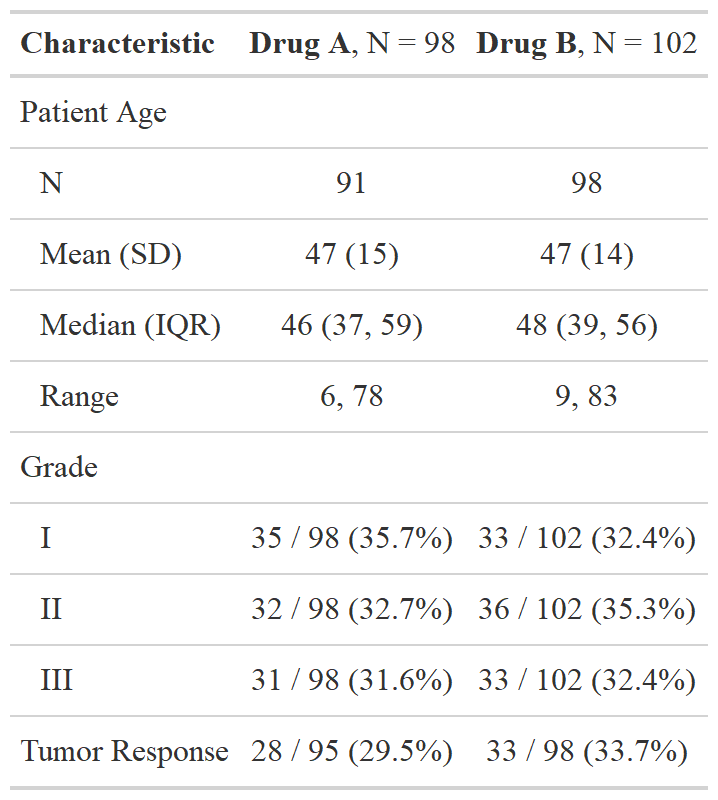
\includegraphics[height=5cm]{summary_plus.png}
  \centering
\end{figure}

\textbf{A note about notation:}
Throughout the gtsummary package, you'll find function arguments that accept a list of formulas (or a single formula) as the input.
In the example above, the label for the age variable was updated using \texttt{label = age $\sim$ "Patient Age"}---equivalently, \texttt{label = list(age $\sim$ "Patient Age")}.
To select groups of variables, utilize the select helpers from the tidyselect\citep{tidyselect} and gtsummary.
Above, \texttt{all\_continuous()} was utilized to change the summary statistics for all continuous variables. 
Similarly, users may utilize \texttt{all\_categorical()} (from gtsummary), or any of the tidyselect helpers used throughout the tidyverse\citep{tidyverse} package, such as \texttt{starts\_with()}, \texttt{contains()}, etc.

The gtsummary package has several functions to add information or statistics to \texttt{tbl\_summary()} tables.

% code for tbl_summary() with arguments
\captionsetup[table]{labelformat=empty,skip=1pt}
\begin{longtable}{ll}
\toprule
Function & Description \\ 
\midrule
\texttt{add\_p()} & add \emph{p}-values to the output comparing values across groups \\ 
\texttt{add\_overall()} & add a column with overall summary statistics \\ 
\texttt{add\_n()} & add a column with N (or N missing) for each variable \\ 
\texttt{add\_difference()} & add column for difference between two group, confidence interval, and \emph{p}-value \\ 
\texttt{add\_stat\_label()} & add label for the summary statistics shown in each row \\ 
\texttt{add\_stat()} & generic function to add a column with user-defined values \\ 
\texttt{add\_q()} & add a column of \emph{q}-values to control for multiple comparisons \\ 
\bottomrule\caption{\label{tab:caption}Table 3. \texttt{tbl\_summary()} functions to add information}\\

\end{longtable}



In the example below the number of non-missing observations is reported for each variable, as well as a p-value comparing the values between the treatment.
The \texttt{add\_p(pvalue\_fun=)} argument accept both a proper function as well the formula shortcut notation used through the tidyverse packages.

\begin{example}
trial %>%
  select(age, grade, response, trt) %>%
  tbl_summary(by = trt, missing = "no") %>%
  add_n() %>%
  add_p(test = all_continuous() ~ "t.test",
        pvalue_fun = ~style_pvalue(., digits = 2))

\end{example}
\begin{figure}[h!]
  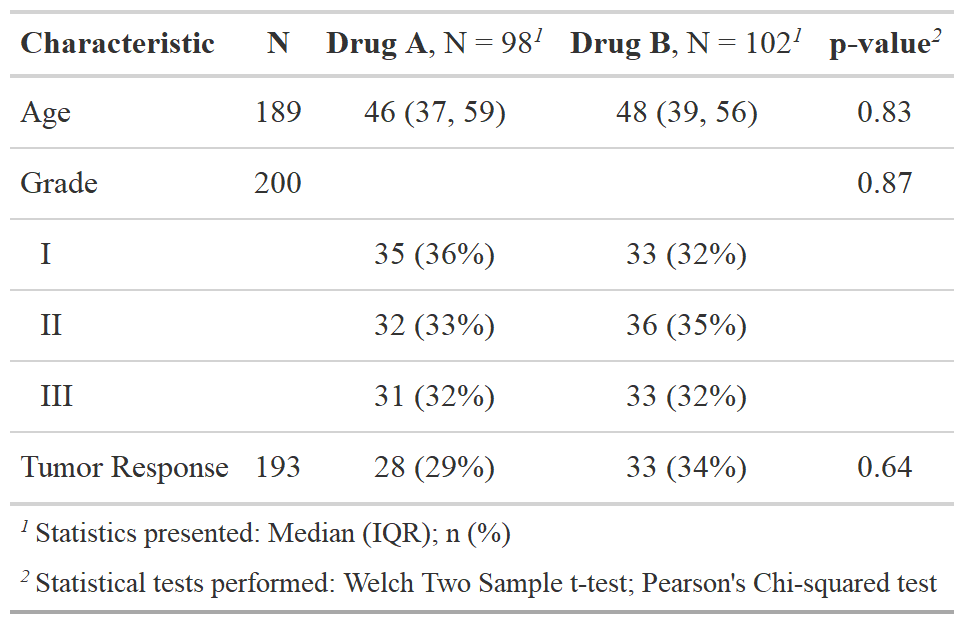
\includegraphics[height=5cm]{summary_plus_plus.png}
  \centering
\end{figure}

\subsection{\texorpdfstring{\texttt{tbl\_svysummary()}}{tbl\_svysummary()}}

The \texttt{tbl\_svysummary()} function is very similar to \texttt{tbl\_summary()} except a survey object is supplied rather than a data frame.

\begin{example}
# create weighted survey object, keep only two counties
data(api, package = "survey")
svy_api <- 
  survey::svydesign(id = ~dnum, weights = ~pw, data = apiclus1, fpc = ~fpc) %>%
  subset(cname %in% c("Alameda", "Los Angeles"))

# summarize data
svy_api %>%
  tbl_svysummary(by = cname, 
                 include = c(growth, target, cname),
                 label = list(growth ~ "Growth",
                              target ~ "Target")) %>%
  add_p()
\end{example}
\begin{figure}[H]
  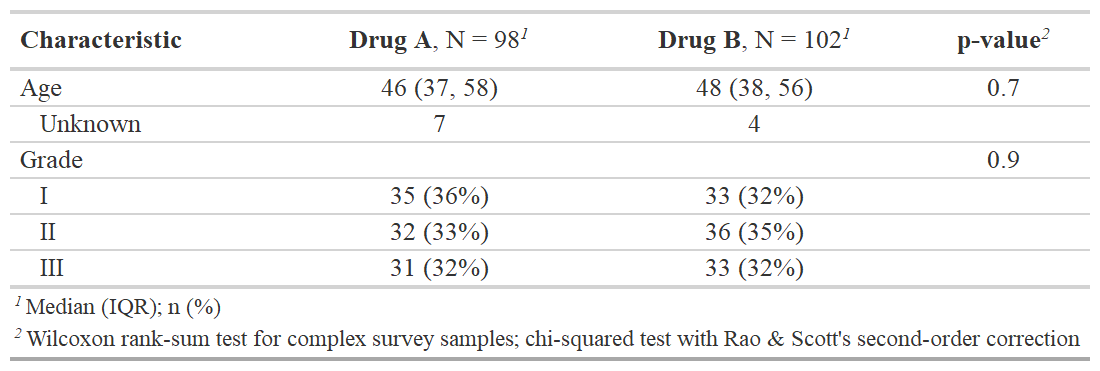
\includegraphics[height=4cm]{svysummary.png}
  \centering
\end{figure}

\subsection{\texorpdfstring{\texttt{tbl\_cross()}}{tbl\_cross()}}

The \texttt{tbl\_cross()} function continues using similar syntax as the previous functions, resulting in a cross tabulation table ready for publication. 

\begin{example}
trial %>%
  tbl_cross(row = stage, col = trt, percent = "cell") %>%
  add_p(source_note = TRUE)
\end{example}
\begin{figure}[h!]
  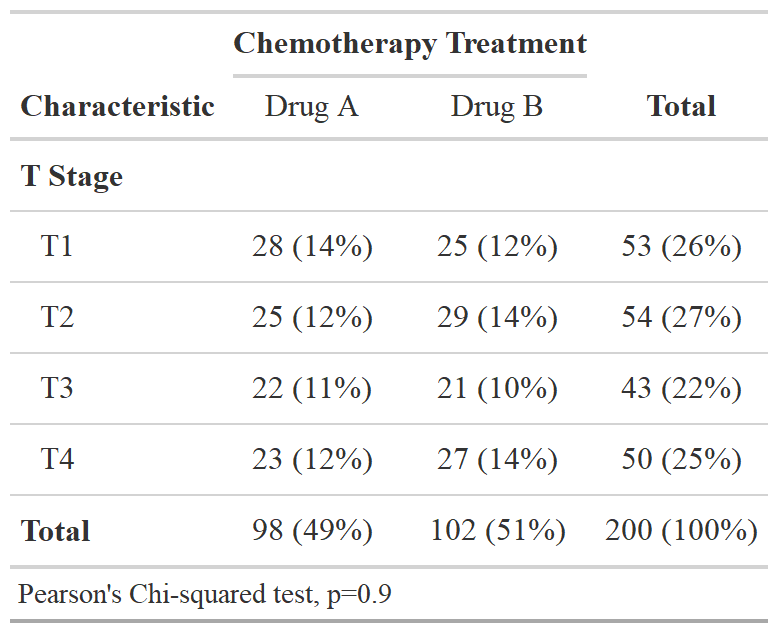
\includegraphics[height=4cm]{cross.png}
  \centering
\end{figure}

\subsection{\texorpdfstring{\texttt{tbl\_survfit()}}{tbl\_survfit()}}

The \texttt{tbl\_survfit()} parses and tabulates n-year survival and survival percentile estimates from \texttt{survival::survfit()} objects.

\begin{example}
library(survival)

list(survfit(Surv(ttdeath, death) ~ trt, trial),
     survfit(Surv(ttdeath, death) ~ grade, trial)) %>%
  tbl_survfit(times = c(12, 24),
              label_header = "**{time} Month**") %>%
  add_p()
\end{example}

% TODO: I do not understand why this isn't being placed below the code! https://www.overleaf.com/learn/latex/Positioning_of_Figures
\begin{figure}[h!]
  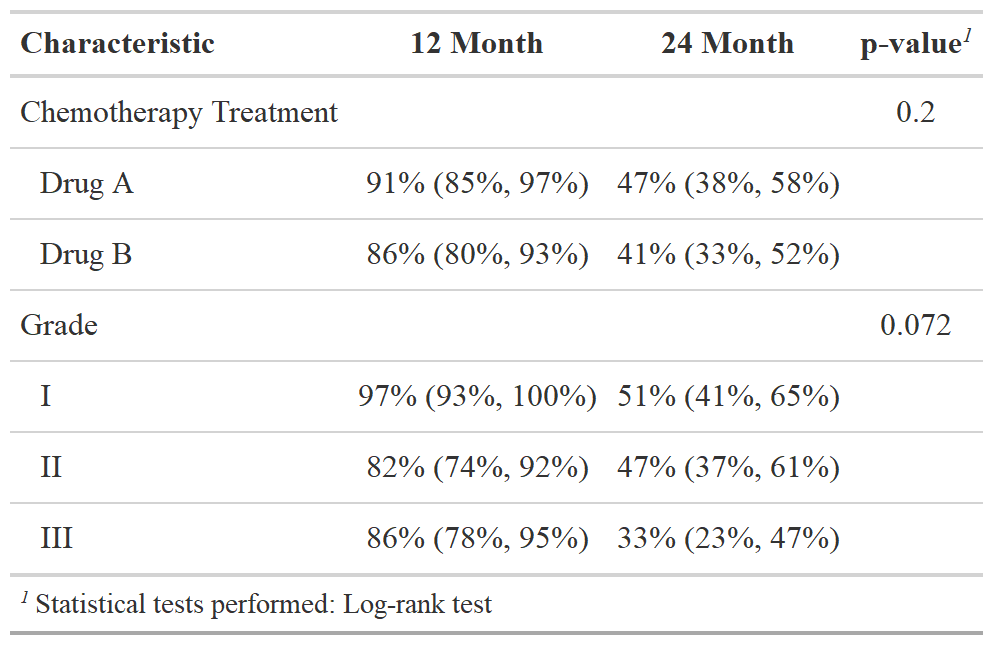
\includegraphics[height=4cm]{survfit.png}
  \centering
\end{figure}

\subsection{Customization}

The gtsummary package includes functions specifically made to modify and format the summary tables.
These functions work with any table constructed with gtsummary.
Most common uses are changing the column headers and footnotes.

% adding table describing fns for customization
\captionsetup[table]{labelformat=empty,skip=1pt}
\begin{longtable}{ll}
\caption{\label{tab:} Functions to style and modify gtsummary tables}\\
\toprule
Function & Description \\ 
\midrule
\texttt{modify\_header()} & update column headers \\ 
\texttt{modify\_footnote()} & update column footnote \\ 
\texttt{modify\_spanning\_header()} & update spanning headers \\ 
\texttt{modify\_caption()} & update table caption/title \\ 
\texttt{bold\_labels()} & bold variable labels \\ 
\texttt{bold\_levels()} & bold variable levels \\ 
\texttt{italicize\_labels()} & italicize variable labels \\ 
\texttt{italicize\_levels()} & italicize variable levels \\ 
\texttt{bold\_p()} & bold significant p-values \\ 
\bottomrule
\end{longtable}



The gtsummary package utilizes the gt package\citep{gt} to print the summary tables.
The gt package exports approximately one hundred functions to customize and style tables.
When you need to add additional details or styling not available within gtsummary, use the \texttt{as\_gt()} to convert the gtsummary object to gt and continue customization.

\begin{example}
trial %>%
  select(age, grade, trt) %>%
  tbl_summary(by = trt, missing = "no") %>%  
  add_overall() %>%    
  add_p() %>%      
  add_stat_label() %>%     
  modify_header(label ~ "**Variable**") %>%   
  modify_spanning_header(c(stat_1, stat_2) ~ "**Treatment Recieved**") %>%  
  as_gt() %>% 
  gt::tab_header(   
    title = gt::md("**Table 1. Patient Characteristics**"),
    subtitle = gt::md("_Highly Confidential_")
  ) %>%
  gt::tab_source_note("Data updated June 26, 2015")   
\end{example}
\begin{figure}[h!]
  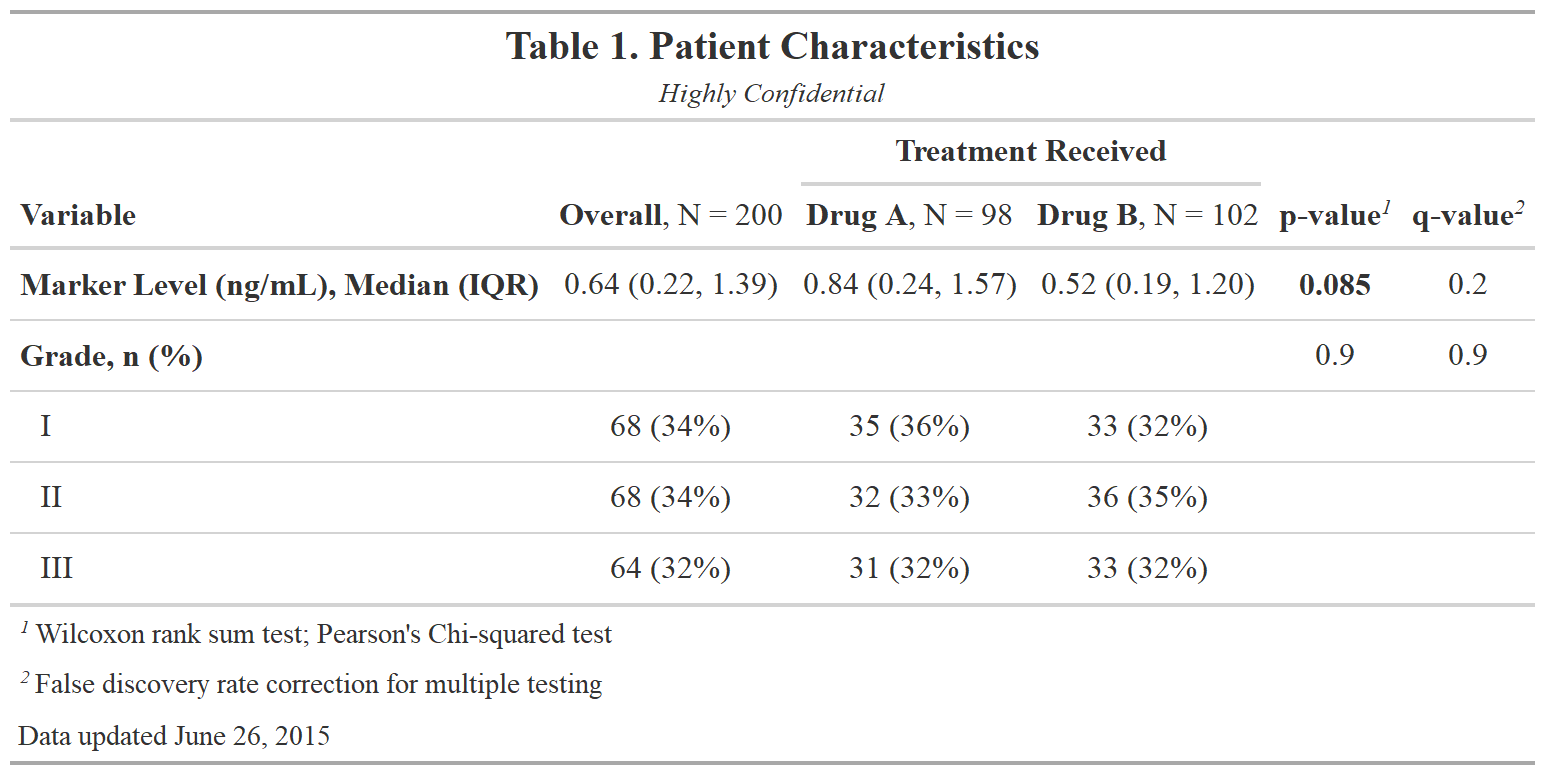
\includegraphics[height=4cm]{custom.png}
  \centering
\end{figure}

\section{Model Summaries}

Regression modelling is one of the most common tools of medical researchers.
The gtsummary has two functions to assist researchers and analysts to prepare tabular summaries of regression models: \texttt{tbl\_regression()} and \texttt{tbl\_uvregression()}.

\subsection{\texorpdfstring{\texttt{tbl\_regression()}}{tbl\_regression()}}

The \texttt{tbl\_regression()} function takes a regression model object in R and returns a formatted table of regression model results. 
Like \texttt{tbl\_summary()}, \texttt{tbl\_regression()} creates highly customizable analytic tables with sensible defaults.
Common regression models, such as logistic regression and Cox proportional hazards regression, are automatically identified and the tables headers are pre-filled with appropriate column headers (i.e. Odds Ratio and Hazard Ratio).

In the example below, the logistic regression model is summarized with \texttt{tbl\_regression()}.
Note that reference row for Grade I has been added, and the variable labels have been carried through into the table.
Using \texttt{exponentiate = TRUE} exponentiates the regression coefficients yielding the odds ratios.
The helper function \texttt{add\_global\_p()} was used to replace the p-values for each term with the global p-value for grade.

\begin{example}
glm(response ~ age + grade, trial, family = binomial) %>%
  tbl_regression(exponentiate = TRUE) %>%
  add_global_p()
\end{example}

\begin{figure}[h!]
  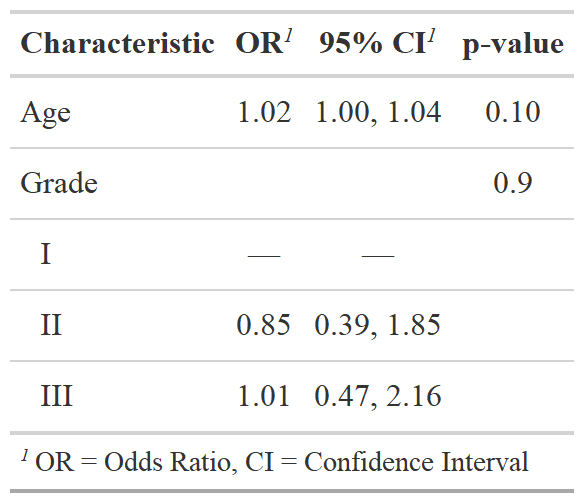
\includegraphics[height=4cm]{regression.png}
  \centering
\end{figure}

The \texttt{tbl\_regression()} function leverages the huge effort behind the broom package's \texttt{tidy()} function to perform the initial formatting of the regression object\citep{broom}.
Because \texttt{tbl\_regression()} utilizes \texttt{broom::tidy()}, there are many model types that are supported out of the box, such as \texttt{lm()}, \texttt{glm()}, \texttt{lme4::lmer()}, \texttt{lme4::glmer()}, \texttt{geepack::geeglm()}, \texttt{survival::coxph()}, \texttt{survival::survreg()}, \texttt{survival::clogit()}, \texttt{nnet::multinom()}, \texttt{rstanarm::stan\_glm()}, models built with the mice package[add ref]and more. The gtsummary package also contains a handful of custom tidiers to report standardized coefficients and bootstrapped confidence intervals.

\subsection{\texorpdfstring{\texttt{tbl\_uvregression()}}{tbl\_uvregression()}}

The \texttt{tbl\_uvregression()} function is a wrapper for \texttt{tbl\_regression()} that is useful when you need a series of univariate regression models.
The user passes a data frame to \texttt{tbl\_uvregression()}, indicates what the outcome is, what regression model to run, and the function will return a beautifully formatted table of stacked univarate regression models.

\begin{example}
trial %>%
  select(response, age, grade) %>%
  tbl_uvregression(
    y = response, 
    method = glm,
    method.args = list(family = binomial),
    exponentiate = TRUE,
    pvalue_fun = ~style_pvalue(., digits = 2)
  ) %>%
  add_nevent() %>%
  add_global_p()
\end{example}

\begin{figure}[h!]
  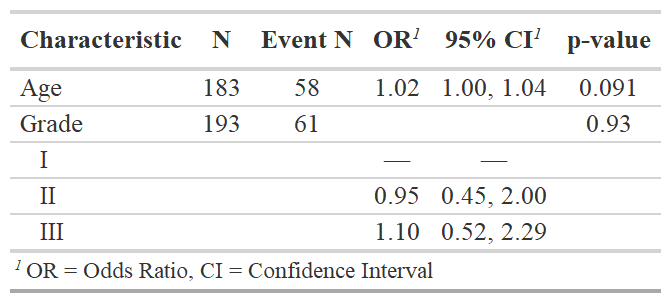
\includegraphics[height=4cm]{uvregression.png}
  \centering
\end{figure}

\section{Inline Reporting}

Reproducible reports are an important part of good practices.
We often need to report the results from a table in the text of an R markdown report.
Inline reporting has been made simple with \texttt{inline\_text()}.
The function reports statistics from gtsummary tables inline in an R markdown document.

Imagine you need to report the results for age from the univariate table above.
Typically, the odds ratio, confidence interval, and p-value would be hard-coded into a report, which can lead to reproducibility issues if the data is updated and the hard-coded statistics are not amended.
A simple call to the \texttt{inline\_text()} function will dynamically add the model results to a an Rmarkdown report.

\begin{quote}
The odds ratio for age was \texttt{\textasciigrave{}r\ inline\_text(uvreg,\ variable\ =\ age)\textasciigrave{}}.
\end{quote}

Here's how the line will appear in your report.

\begin{quote}
The odds ratio for age was 1.02 (95\% CI 1.00, 1.04; p=0.091).
\end{quote}

The default pattern to display for a regression table is \texttt{"\{estimate\} (\{conf.level*100\}\% CI \{conf.low\}, \{conf.high\}; \{p.value\})"} (again using glue syntax), and can be modified with the \texttt{inline\_text(pattern=)} argument. 

\section{Merging and Stacking}

\section{Themes}

The default styling (e.g. statistics displayed in \texttt{tbl\_summary()}, how p-values are rounded, decimal separator, and more) follow the reporting guidelines from European Urology, The Journal of Urology, Urology, and the British Journal of Urology International\citep{assel2019guidelines}.
However, you'll likely submit to another journal, or your personal preferences different from the defaults.
The gtsummary package is unique from other table building packages in the ability to set fine-grained customization defaults with themes. 
Themes were created to make these customizations easy to navigate and reuse across documents or projects. 
Several ready built themes are available in the package.
With themes, users can control default settings for existing functions (e.g. always present means instead of medians in \texttt{tbl\_summary()}), as well as other changes that are not modifiable with function arguments.

For example, using the theme for New England Journal of Medicine, large p-values are rounded to two decimal places and confidence intervals are shown as \texttt{"lb to ub"} instead of \texttt{"lb, ub"}.

\begin{example}
theme_gtsummary_journal("nejm")

glm(response ~ age + grade, trial, family = binomial) %>%
  tbl_regression(exponentiate = TRUE)
\end{example}

\begin{figure}[h!]
  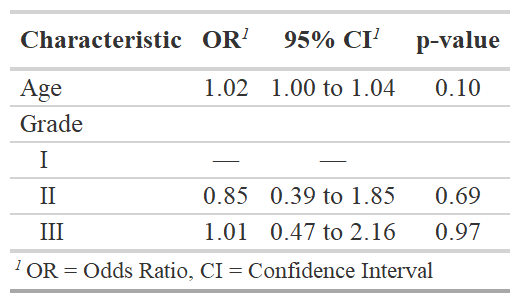
\includegraphics[height=4cm]{nejm.png}
  \centering
\end{figure}

The themes are an evolving feature and we welcome additions of new journals and other useful themes.
A full glossary of customizable theme elements is available in the package documentation (\url{http://www.danieldsjoberg.com/gtsummary/articles/themes.html}).

\section{Print Engines}

SHOULD WE JUST REMOVE THIS SECTION?!

\begin{figure}[h!]
  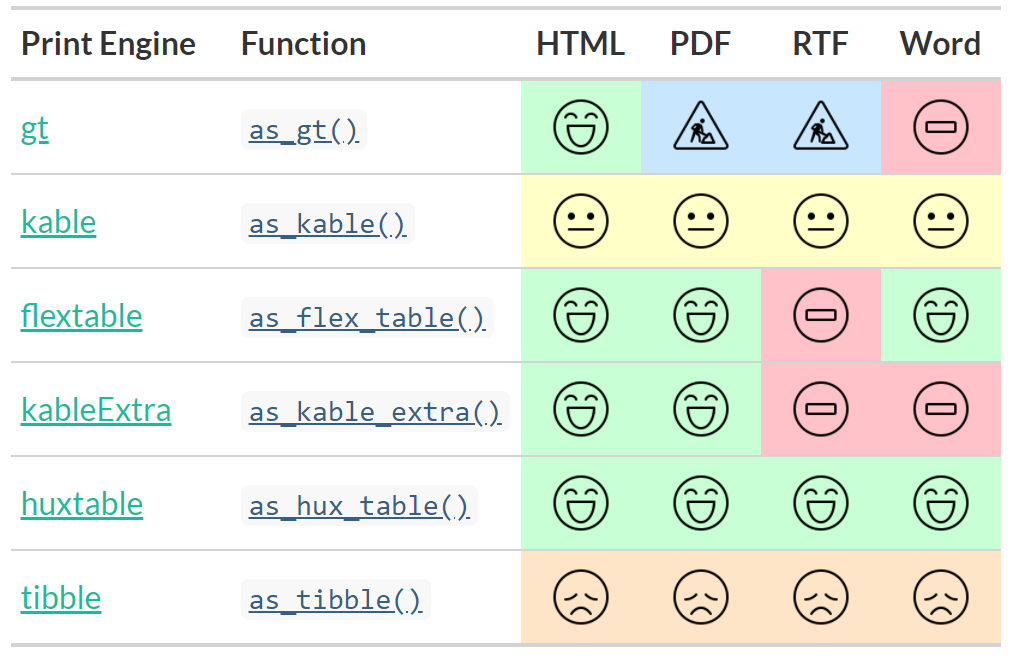
\includegraphics[height=4.5cm]{print_engines.png}
  \centering
\end{figure}

\section{Summary}

\bibliography{RJreferences}

\address{Daniel D. Sjoberg\\
  Memorial Sloan Kettering Cancer Center\\
  1275 York Ave., New York, New York 10022\\
  USA\\
  ORCID 0000-0003-0862-2018\\
  \email{sjobergd@mskcc.org}}

\address{Karissa Whiting\\
  Memorial Sloan Kettering Cancer Center\\
  1275 York Ave., New York, New York 10022\\
  USA\\
  ORCID 0000-0002-4683-1868\\
  \email{whitingk@mskcc.org}}

\address{Michael Curry\\
  Memorial Sloan Kettering Cancer Center\\
  1275 York Ave., New York, New York 10022\\
  USA\\
  ORCID 0000-0002-0261-4044\\
  \email{currym1@mskcc.org}}
